% Note that the a4paper option is mainly intended so that authors in
% countries using A4 can easily print to A4 and see how their papers will
% look in print - the typesetting of the document will not typically be
% affected with changes in paper size (but the bottom and side margins will).
% Use the testflow package mentioned above to verify correct handling of
% both paper sizes by the user's LaTeX system.
%
% Also note that the "draftcls" or "draftclsnofoot", not "draft", option
% should be used if it is desired that the figures are to be displayed in
% draft mode.
%
%\documentclass[journal,draft]{IEEEtran}
\documentclass[journal]{IEEEtran}
%
% If IEEEtran.cls has not been installed into the LaTeX system files,
% manually specify the path to it like:
% \documentclass[journal]{../sty/IEEEtran}

% *** MISC UTILITY PACKAGES ***

% *** CITATION PACKAGES ***
%
\usepackage{cite}

% *** GRAPHICS RELATED PACKAGES ***
%
\usepackage[dvips]{graphicx}
\usepackage{amsmath}
\usepackage{dsfont}     % for \mathds support

\usepackage[ansinew]{inputenc} %WINDOWS character support

% correct bad hyphenation here
\hyphenation{op-tical net-works semi-conduc-tor}

\newcommand{\bvec}[1]{\ensuremath{\mathbf{#1}}}
\newcommand{\buvec}[1]{\ensuremath{\mathbf{\hat{#1}}}}
\newcommand{\bmat}[1]{\ensuremath{[\mathbf{#1}]}}
\newcommand{\vect}[1]{\boldsymbol{#1}}          % vector
\newcommand{\uvect}[1]{\hat{\boldsymbol{#1}}} % unit vector

\DeclareMathOperator{\spn}{span}

\begin{document}
%
% paper title
% can use linebreaks \\ within to get better formatting as desired
\title{Efficient Parametric Finite Element Analysis of Passive Microwave Devices Using a Domain Decomposition - Model Order Reduction Approach}

\author{Stefano~Selleri,~\IEEEmembership{Senior Member,~IEEE},
    Ortwin Farle, Giacomo Guarnieri, Markus L�sch, \\
    Giuseppe Pelosi,~\IEEEmembership{Fellow,~IEEE},
    Romanus Dyczij-Edlinger,~\IEEEmembership{Member,~IEEE}
 %       Stefano~Selleri,~\IEEEmembership{Senior Member,~IEEE,}
\thanks{Manuscript received Month DD, YYYY; revised Month DD, YYYY.}
\thanks{This work has been developed within a Vigoni Italy-Germany researcher exchange programme financed for years 2007-2008.}
\thanks{S. Selleri and G. Pelosi are with
Department of Electronics and Telecommunications,
University of Florence, Via C. Lombroso 6/17 - 50134 - Florence, Italy}%
\thanks{O. Farle, M. L�sch and R. Dyczij-Edlinger are with
Lehrstuhl f\"ur Theoretische Elektrotechnik, Universit\"at des
Saarlandes
D-66041 Saarbr\"ucken, Germany}%
\thanks{G. Guarnieri
Galileo Avionica S.p.A. - BU Radar Systems Antennas,
via A. Einstein, 35 - 50013 - Campi Bisenzio (FI) Italy}%
}

% The paper headers
\markboth{IEEE Transactions on Microwave Theory and Techniques,~Vol.~VV, No.~N,
Month~YYYY}{Nosotros: The Title...}


% make the title area
\maketitle

\begin{abstract}
In this paper we present a new methodology for efficient parametric finite element analysis.
Since broadband parameter variations demand for increased numerical robustness,
we propose the use of a multipoint order reduction method.
These come along with high computational costs for constructing the projection space.
Since most of the considered parameters are local,
this means only a small part of the field domain changes,
the generation process of the reduced order model can be accelerated by incorporating a domain decomposition approach.
We present several examples that demonstrate the efficacy of the proposed technique.
\end{abstract}

\begin{IEEEkeywords}
Finite element methods, Reduced order systems, Domain decomposition
\end{IEEEkeywords}

\section{Introduction}
\IEEEPARstart{T}{he} finite element (FE) method is very well known for its flexibility and reliability
as well as its relatively high computational times.
%This is a problem when frequency sweeps and material parameter sweeps have to be accounted for
%and, indeed, several techniques have been proposed to get faster sweeps in frequency \cite{Bracken98} %\cite{Pol97}
%and,
%in material parameters \cite{Far06,FarIP}.
This can become a major issue,
if the solution is sought as a function of a multidimensional parameter space.
Possible applications are optimization scenarios or parametric studies.
Typical parameters include frequency \cite{Bracken98},
material properties \cite{Far06} and geometry parameters \cite{Daniel2004}.
A promising candidate for efficiently handling these parameter dependent systems is model order reduction (MOR) \cite{Antoulas2005}.
Almost all of the modern MOR approaches are projection based.
This means,
the original system,
with up to millions of degrees of freedoms,
is projected onto a low dimensional subspace of global shape functions,
thus drastically reducing the dimension of the model with introducing only a minor additional approximation error.
The number of global shape functions is typically between ten and a few hundred.
The various order reduction methods mainly differ in the projection spaces
and the way the projection matrices are computed numerically.
MOR algorithms can either be characterized as a single point or a multipoint method.
Most single point methods \cite{Gunupudi2002,Daniel2004} are of moment matching type.
This means,
the resulting reduced order model (ROM) matches the derivatives of the transfer function of the full model
at a given expansion point up to a certain order.
Since ROM and original model share the same parameterized structure,
the ROM is a multidimensional Pad� approximation \cite{Weile1999}.
The key feature of single point methods is the fact,
that the system matrix of the full model only has to be factorized in the expansion point,
so one matrix factorization is sufficient.
This advantage looses importance as soon as iterative solvers have to be used.
Although in recent time,
progress has been made in improving the numerical stability of single point methods for the multi parameter case
\cite{Codecasa2005,Feng2005,FarIP},
multipoint methods like \cite{Weile2001,PrudHomme02} are still numerically more robust.
Additionally they usually result in ROMs of smaller dimension,
as demonstrated in \cite{Schultschik2008} for the single parameter case.
The main drawback of multipoint approaches
is the need for solving the full FE system at several points in the parameter space.
This is especially true for the method of proper orthogonal decomposition (POD) \cite{Holmes96},
where the projection basis is subsequently reduced by a low rank approximation,
to achieve a further decrease in ROM dimension.


%Despite this high computation costs for ROM generation we here propose to use

%here: multipoint
%cons: high computation costs for ROM generation

%{\bf Bla bla bla (Ortwin\ldots)}
%Most of these techniques can be characterized as model order reduction (MOR) methods.

%These techniques allow for very fast solutions once the reduced order model (ROM) is obtained,
%nevertheless to obtain such a model the complete FE model must be built and solved once for single-point methods,
%more than once for the multipoint methods,
%these latter {\bf bla bla bla}.
%These computations,
%for as few as they might be,
%are still very time consuming.

Another approach to the problem of speeding up FE solution
which is rapidly gaining popularity is that of domain
decomposition (DD) methods. DD is indeed a very general
approach encompassing a broad category of techniques based on
the ``divide-and-conquer'' principle applied to a global large
boundary value problem (BVP), as those typical of wave
electromagnetic engineering. In a very general approach DD can
be seen as a procedure to gather information at the inner
boundaries $\Gamma$ of a partition of a generic domain $\Omega$
so as to be able to define well-posed problems on each single
subdomain \cite{Her03}.

The most attractive feature of these methods is the possibility
to take into account very large electromagnetic domains, moving
up the limit of electromagnetic problems treatable via
full-wave methods and providing parallelization as a side
effect \cite{Cho96}.

Indeed many well established approaches implemented in the
past can be reconducted to the DD paradigm, starting from those
based on a subdivision of the domain into parts which are coupled
via a modal expansion \cite{Lee97, Rub99, Rub01, Lim01, Mar03}.

A more general and powerful approach is that of subdividing the
domain without the need to define interfaces between the
subdomains regular enough to allow a modal expansion, among
these we can cite Schwartz methods \cite{Smi96} and its
developments \cite{Her01}, project decomposition methods
\cite{Ago94}, Mortar \cite{Ber94} and finite element tear and
interconnect (FETI) methods \cite{Her00}. Many of these
techniques have been recently applied to engineeristic
electromagnetic problems \cite{Bal04,Mat07,Zha06,Wol07}.

This paper will present a FE based domain decomposition
technique based on the Schur complement technique \cite{Saa03}
intended as a fast procedure to obtain the solutions needed to
apply a multipoint MOR solution. In particular the domain
partitioning will be performed so as to concentrate all the
materials on which a parametric sweep is to be performed
into a single, not necessarily simply connected, subdomain.

Results will be presented on simple passive microwave devices
which can either be considered as H-plane devices. This
is not a limit of the approach, which can be trivially extended
to 3D but is rather a choice done to more easily present
results.

In following Section II the problem will be defined, the FE
formulation itself will not be discussed in detail as it is
well represented in literature \cite{Pel98,Rub01}. Section III
will present the details of the proposed DD approach and the
derivation of the system to which MOR will be applied in
subsequent Section IV. Section V will present numerical results
over a couple of test cases, stressing the gain in CPU time
attained. Finally Section VI will draw the conclusions.


\section{Statement of the problem}
The problem to which the proposed combined DD-MOR technique
will be applied is that of the FE solution of a generic P-port
device (Fig.~\ref{f:statement}).
%For the sake of simplicity, and without any loss of generality, only
%devices uniform either with respect to the E-plane or the H-plane will be
%considered. With this hypothesis a 2D FE approach is possible.
For the sake of simplicity, and without any loss of generality, only
devices uniform with respect to the H-plane will be
considered. With this hypothesis a 2D FE approach is possible.
\begin{figure}[!t]
  \centering
  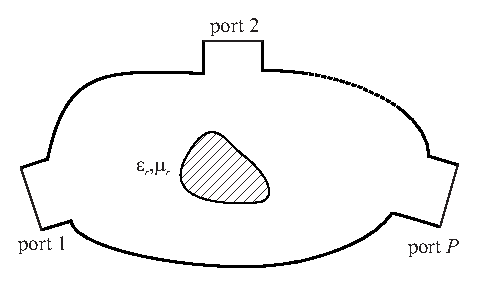
\includegraphics[scale = 0.9]{figs/statement.eps}
  \caption{Geometry of a generic $P$-port device comprising some
  dielectric region.}
  \label{f:statement}
\end{figure}
The FE formulation is then scalar and concerns a
single field component. To fully define the boundary value
problem suitable conditions at the device ports need to
be considered. These are usually obtained by enforcing a
modal expansion at the port, deriving formulations
which are based, for example, on the concept of generalized
scattering matrix (GSM) \cite{Pel98} or on the concept of
generalized admittance matrix (GAM) \cite{Rub01}.

Previous researches in this field \cite{Who08} adopted the GSM approach,
but the presence of a non-polynomial dependency from frequency in the modal coupling matrices
makes this formulation less suitable for MOR,
if frequency is to be considered among sweep parameters.
On the other hand the GAM formulation does not present this issue
and therefore is exploited when expand pure material parameter sweeps \cite{Sel08,Sel08b} to frequency parameterization.

The considered boundary problem reads as
%
\begin{subequations} \label{eq:BVP}
\begin{align}
  &\nabla_t \cdot \mu_r^{-1} \nabla_t E_z + k_0^2 \varepsilon_r E_z = 0 &\text{in } \Omega \\
  &E_z = 0 &\text{on } \Gamma_E \\
  &\uvect n \cdot \mu_r^{-1} \nabla_t E_z = 0 &\text{on } \Gamma_H \\
  &\uvect n \cdot \mu_r^{-1} \nabla_t E_z = j k_0 \eta_0 \uvect e_z \cdot \bar{\vect H}_t \times \uvect n &\text{on } \Gamma_P
\end{align}
\end{subequations}
%
where $\Omega$ denotes the field domain with
boundary $\partial \Omega = \Gamma$ consisting of three disjoint parts
$\Gamma = \Gamma_E \cup \Gamma_H \cup \Gamma_P$.
In \eqref{eq:BVP},
$E_z(x,y)$ stands for the $z$ component of the electrical field,
$\varepsilon_r(x,y)$ for the relative electric permittivity,
$\mu_r(x,y)$ for the relative magnetic permeability,
$\nabla_t = \uvect e_x \partial_x + \uvect e_y \partial_y$ for the transversal nabla operator,
$k_0$ and $\eta_0$ for the free space wave number and characteristic impedance, respectively.
The outward pointing unit vector on surface $\Gamma$ is given by $\uvect n$.
With $\bar{\vect H}_t$ we denote the transversal magnetic field of the excited waveguide mode.


\section{Domain Decomposition Approach} \label{sec:DdApproach}
Fig.~\ref{f:dd} sketches a generic 2-port waveguide device on
H plane. The whole device domain $\Omega$ is subdivided in an
arbitrary number $N$ of non-overlapping subdomains $\Omega_i$
so that
%
\begin{equation}
\Omega = \bigcup_{i=1}^N \Omega_i; \;\;\;\; \Omega_i \cap \Omega_j = \emptyset
\;\; \forall i\neq j.
\label{e:dd}
\end{equation}
%
Each $\Omega_i$ is limited by boundary $\partial \Omega_i$,
which is explicitly divided so as to uniquely identify each
border section between different sub domains. In particular the
portion of $\partial \Omega$ between $\Omega_i$ and the generic
neighboring domain $\Omega_j$ is denoted $\Gamma_{i,j}$. If to
the infinite space outside the domain of the problem, and
outside the feeding waveguide structures, we assign ideally the
index zero then the boundaries of the subdomains which
coincides with the boundary of the problem can be denoted by
$\Gamma_{i,0}$. On these boundary two cases are possible, in
this approach, either there is a Dirichlet or Neumann boundary
condition to be imposed.
\begin{figure}[!t]
  \centering
  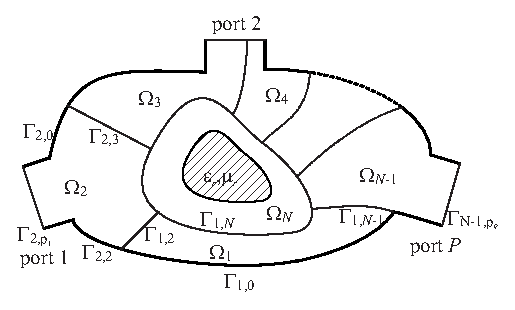
\includegraphics[scale = 0.925]{figs/dd.eps}
  \caption{Geometry of a generic two port device with partitioning in
  sub-domains. For the sake of clarity only a part of the boundaries have been
  explicitly labeled.}
  \label{f:dd}
\end{figure}
On the other hand, boundaries between the generic $\Omega_i$
domain and a feeding waveguide structure, that is on the
generic $p_k$ port, are denoted as $\Gamma_{i,p_k}$. Here a
suitable modal expansion is to be imposed.

It is well known that the FE solution within $\Omega$ leads to a linear
system in the form $\bmat{A}\bvec{x}=\bvec{c}$ and it can be
shown in a DD framework this system can be rewritten as:
%
\begin{equation}
\begin{bmatrix}
\bmat{M}_1 & 0 & \cdots & 0 & {\bmat{E}}_1 \\
0 & \bmat{M}_2 & \cdots & 0 & {\bmat{E}}_2 \\
\vdots & \vdots & \ddots & \vdots \\
0 & 0 & \cdots & \bmat{M}_N & {\bmat{E}}_N \\
{\bmat{E}}_1^T & {\bmat{E}}_2^T &\cdots & {\bmat{E}}_N^T &
{\bmat{C}}
\end{bmatrix}
\begin{bmatrix}
\bvec{x}_1 \\
\bvec{x}_2 \\
\vdots \\
\bvec{x}_N \\
{\bvec{y}} \\
\end{bmatrix}
=
\begin{bmatrix}
0 \\
0 \\
\vdots \\
0 \\
{\bvec{c}}
\end{bmatrix}
\label{e:fullDD}
\end{equation}
%
in which $\bmat{M}_i=\bmat{S}_i-k_0^2\bmat{T}_i$ are the sparse
matrices pertaining to the FEM solution on the inner unknowns
$\bvec{x}_i$ in subdomain $\Omega_i$. On the other hand,
unknowns relative to the boundaries of the subdomains
$\Gamma_{i,j}$ and $\Gamma_{i,p_k}$ are all collected in the
$\bvec{y}$ vector.
Matrices $\bmat{E}_i$ and $\bmat{C}$ are still assembled by resorting to
element stiffness and mass matrices but are relevant to border unknowns. In
particular $\bmat{E}_i$ contains the interaction between inner unknowns of
$\Omega_i$ and unknowns on $\partial \Omega_i$ while $\bmat{C}$ pertains to the
interaction among border unknowns.
It is worth noticing how $\bmat{E}_i$  matrices are very sparse since the
only columns of $\bmat{E}_i$ which are nonzero are those relative to those
entries of $\bvec{y}$ which belong to $\Omega_i$.
Finally matrix $\bmat{C}$ pertains to the interaction between border unknowns.

If an explicit distinction is made among the unknowns pertaining to ports from all
other border unknowns, it is possible to write
%
\begin{equation}
\bvec{y} = \begin{bmatrix}\bvec{y}^{(0)} \\ \bvec{y}^{(p)}\end{bmatrix}
\end{equation}
%
where $\bvec{y}^{(0)}$ contains all the degrees of freedom on
$\Gamma_{i,j}$ $\forall i,j=0,\ldots,N$ while $\bvec{y}^{(p)}$
contains all the degrees of freedom belonging to
$\Gamma_{i,p_k}$ $\forall i=0,\ldots,N$ and $\forall
k=1,\ldots,P$. Matrix $[\bvec{M}]$ of system (\ref{e:fullDD})
can be written in an expanded form as
%
\begin{equation}
\begin{bmatrix}
\bmat{M}_1 & 0 & \cdots & 0 & \bmat{E}_1^{(0)} & \bmat{E}_1^{(p)}\\
0 & \bmat{M}_2 & \cdots & 0 & \bmat{E}_2^{(0)} & \bmat{E}_2^{(p)}\\
\vdots & \vdots & \ddots & \vdots & \vdots \\
0 & 0 & \cdots & \bmat{M}_N & \bmat{E}_N^{(0)} & \bmat{E}_N^{(p)}\\
\bmat{E}_1^{(0)^T} & \bmat{E}_2^{(0)^T} &\cdots & \bmat{E}_N^{(0)^T} &
\bmat{C}^{(0)} & 0 \\
\bmat{E}_1^{(p)^T} & \bmat{E}_2^{(p)^T} &\cdots & \bmat{E}_N^{(p)^T} &
0 & \bmat{C}^{(p)}  \\
\end{bmatrix}.
\label{e:expandedDD}
\end{equation}
%
By defining a suitable projection matrix
%
\begin{equation}
\bmat{B} = \begin{bmatrix}
\bmat{I}_1 & 0 & \cdots & 0 & 0 & 0\\
0 & \bmat{I}_2 & \cdots & 0 & 0 & 0\\
\vdots & \vdots & \ddots & \vdots & \vdots \\
0 & 0 & \cdots & \bmat{I}_N & 0 & 0\\
0 & 0 & \cdots & 0 & \bmat{I}^{(0)} & 0 \\
0 & 0 & \cdots & 0 & 0 & \bmat{P}_1, \ldots \bmat{P}_P  \\
\end{bmatrix}
\label{e:projectionmatrix}
\end{equation}
%
in which $\bmat{I}_i$ are identity matrices of suitable dimensions
while $\bmat{P}_k$ are rectangular $N_{n_{k}} \times N_{m_{k}}$ matrices,
$N_{n_k}$ and $N_{m_k}$ being the number of unknowns and the number of modes on port $k$, respectively.

By applying this projection to the system (\ref{e:fullDD}) a
new system matrix is obtained $\bmat{\tilde{A}} = \bmat{B}^T
\bmat{A} \bmat{B}$ and, explicitly:
%
\begin{equation}
\begin{bmatrix}
\bmat{M}_1 & 0 & \cdots & 0 &  \bmat{\tilde{E}}_1\\
0 & \bmat{M}_2 & \cdots & 0 &  \bmat{\tilde{E}}_2\\
\vdots & \vdots & \ddots & \vdots \\
0 & 0 & \cdots & \bmat{M}_N & \bmat{\tilde{E}}_N\\
\bmat{\tilde{E}}_1^T & \bmat{\tilde{E}}_2^T &\cdots & \bmat{\tilde{E}}_N^T &
\bmat{\tilde{C}} \\
\end{bmatrix}
\label{e:reducedDD}
\end{equation}
%
or, in a more compact form
%
\begin{equation}
\begin{bmatrix}
\bmat{M} & \bmat{\tilde{E}}\\
\bmat{\tilde{E}}^T & \bmat{\tilde{C}} \\
\end{bmatrix}.
\label{e:compactDD}
\end{equation}
%
This system is of reduced dimension since $N_{n_k}>N_{m_k}$. In
particular $N_{m_k}$ can be chosen equal to 1 if only one mode
is propagable and the ports are far enough from the
discontinuities within the device. This is usually undesired
since placing ports far enough from the discontinuity requires
a large domain $\Omega$ to be solved with costly FE, but in the
present DD approach, since this part of the solution will be
computed only once it is worth doing, especially considering
the benefits attained in the MOR, as it will be shown in the
next section.

The solution of (\ref{e:compactDD}) for the boundary unknown
$\bvec{y}$ only can be attained by resorting to the Schur
complement $\bmat{S_c}$ concept:
%
\begin{equation}
\bmat{S_c} =
\bmat{\tilde{C}}-\bmat{\tilde{E}}^T\bmat{M}^{-1}\bmat{\tilde{E}}
\label{e:shur}
\end{equation}
%
\noindent from which
%
\begin{equation}
\bmat{S_c}\bvec{y} = \bvec{c}
\label{e:shursol}
\end{equation}
%
follows immediately.

In a DD framework the Schur complement can be computed on a
subdomain-by-subdomain basis as \cite{Who08}:
%
\begin{equation}
\bmat{S_c} = \bmat{\tilde{C}} - \sum_{i=1}^N
\bmat{\tilde{E}}_i^T\bmat{M}_i^{-1}\bmat{\tilde{E}}_i.
\label{e:shurdd}
\end{equation}
%
It is worth noticing that there is no need of explicitly
computing the inverse of $\bmat{M}_i$ appearing in
(\ref{e:shurdd}), rather the sparse system
%
\begin{equation}
\bmat{M}_i\bmat{F}_i=\bmat{\tilde{E}}_i
\label{e:minverse}
\end{equation}
%
\noindent is solved only for the nonzero columns of
$\bmat{\tilde E}_i$ so that (\ref{e:shurdd}) reduces to
$\bmat{\tilde S} = \bmat{C} - \sum_{i=1}^N \bmat{\tilde
E}_i^T\bmat{F}_i$.

It is apparent from (\ref{e:shurdd}) that, provided that all
structures with parameter-dependent material properties are
placed within a single subdomain, which, without any loss of
generality will considered to be the last, the first $N-1$
components of the Schur complement (\ref{e:shurdd}) can be
computed and stored once for all for each frequency value.

%The last domain can be ideally described by the parameterized
%matrix
%%
%\begin{equation}
%\bmat{M}_N = \bmat{S}_0 - k_0^2\bmat{T}_0 + \sum_{m=0}^M
%\frac{1}{\mu_m}\bmat{S}_m -k_0^2\sum_{m=0}^M \varepsilon_m\bmat{T}_m
%\end{equation}
%%
%where subscript $m=1,\ldots,M$ cycles over the various
%materials on which a parameter sweep is requested.


\section{Model Order Reduction}

To explain our MOR procedure,
we consider an example problem with three parameters:
frequency, relative magnetic permeability $\mu_r$ and relative electric permittivity $\varepsilon_r$ of a subregion.
For sake of brevity and clarity,
we exclude conductor losses and radiation in free space,
but allow for dielectric losses.
Using the E-field formulation \eqref{eq:BVP},
we end up with a parameterized FE system of the form
%
\begin{equation}
    \left( \bmat{S}(\mu_r^{-1}) - k_0^2 \bmat{T}(\varepsilon_r) \right) \bvec{x} = \beta(k_0) \bvec{b} \label{eq:paramSys}
\end{equation}
%
where $\bmat{S}(\mu_r^{-1}) \in \mathds{C}^{n \times n}$ and $\bmat T(\varepsilon_r) \in \mathds{C}^{n \times n}$
denote the mass and stiffness matrix, respectively,
and $k_0$ stands for the free-space wavenumber.
Note that the normalization coefficient $\beta$ shows the only frequency dependence of the right hand side.
The vector $\bvec b$ is constant,
since we are only considering TE or TM modes for excitation \cite{Rub01}.
Introducing the parameters
%
\begin{align} \label{eq:s1}
    s_1 &= k_0^2, &
    s_2 &= \mu_r^{-1}, &
    s_3 &= \varepsilon_r
\end{align}
%
gives for the system matrices
%
\begin{align}
    \bmat{S}(\mu_r^{-1}) &= \bmat{S} + s_2 \bmat{S}^{\mu} \\
    \bmat{T}(\varepsilon_r) &= \bmat{T} + s_3 \bmat{T}^{\varepsilon} \label{eq:parmDepMassMat}
\end{align}
%
where $\bmat{S}^{\mu}$ and $\bmat{T}^{\varepsilon}$ denote the stiffness and mass matrix, respectively,
of the subregion in which the material parameters vary,
whereas $\bmat{S}$ and $\bmat{T}$ belong to the parameter independent parts.
Plugging \eqref{eq:s1} - \eqref{eq:parmDepMassMat} into \eqref{eq:paramSys}
results in a polynomially parameterized linear system of equations of the form
%
\begin{equation} \label{eq:polyParamSys}
\begin{split}
    \left( \bmat{A}_{000} + s_1 \bmat{A}_{100} + s_2 \bmat{A}_{010} + s_1 s_3 \bmat{A}_{101} \right) \bvec x = \beta(s_1) \bvec b
\end{split}
\end{equation}
%
where
%
\begin{subequations}
\begin{align}
    \bmat{A}_{000} &= \bmat{S}, &
    \bmat{A}_{100} &= -\bmat{T} \\
    \bmat{A}_{010} &= \bmat{S}^{\mu}, &
    \bmat{A}_{101} &= \bmat{T}^{\varepsilon}.
\end{align}
\end{subequations}
%\begin{align}
%    \bmat{A}_{000} &= \bmat{S} \\
%    \bmat{A}_{100} &= -\bmat{T} \\
%    \bmat{A}_{010} &= \bmat{S}^{\mu} \\
%    \bmat{A}_{101} &= \bmat{T}^{\varepsilon}.
%\end{align}
%
%In \eqref{eq:polyParamSys} we omitted the $\beta(s_1)$ dependence of the right hand side,
%since a scaling of the right hand side corresponds to the same scaling of the solution vector,
%and so can be taken into account by a simple post-processing step.
Linear systems of equations whose system matrix is parameterized by polynomials in $m$ scalar parameters
$s_1, \dots s_m$ with a maximum polynomial degree of $M$,
in general take the form
%
\begin{align} \label{eq:genPolyParamMod}
	\left( \sum_{| \alpha | = 0}^{| \alpha | \leq M} \bvec s^{\alpha} \bmat A_{\alpha} \right) \bvec x (\bvec s) &= \beta(s_1) \bvec b
\end{align}
%
where  $\alpha = (\alpha_1, \alpha_2, \dots, \alpha_m)$ is a multi-index with $\alpha_i \geq 0$.
We use the following conventions
%
\begin{align}
	| \alpha | &= \sum_{i=1}^m \alpha_i, &
	\bvec s^{\alpha} &= \prod_{i=1}^m s_i^{\alpha_i}.
\end{align}
%
A ROM of \eqref{eq:genPolyParamMod} is constructed
by restricting $\bvec x$ onto a low dimensional subspace of global shape functions.
Following the reduced-basis method of \cite{PrudHomme02} and \cite{Nguyen05},
shape functions $\bvec q_1, \dots , \bvec q_p$ span the space of solutions of the full model \eqref{eq:genPolyParamMod}
at expansion points $\bvec s_1, \dots , \bvec s_p$ in the parameter space
%
\begin{align} \label{eq:ProjVecEqSolVec}
    \spn \{ \bvec q_1, \dots , \bvec q_p \} = \spn \{ \bvec x ( \bvec s_1), \dots , \bvec x ( \bvec s_p ) \}.
\end{align}
%
Applying a Galerkin projection onto the space of global shape functions,
we get from \eqref{eq:genPolyParamMod} a ROM exhibiting the same parameterized structure
%
\begin{align} \label{eq:genPolyParamModROM}
	\left( \sum_{| \alpha | = 0}^{| \alpha | \leq M} \bvec s^{\alpha} \hat{ \bmat A}_{\alpha} \right) \hat{\bvec x} (\bvec s) &= \beta(s_1) \hat{\bvec b}
\end{align}
%
where
\begin{align}
	\hat{ \bmat A}_{\alpha} &= \bmat Q^H \bmat A_{\alpha} \bmat Q \label{eq:projMatr}\\
	\hat{ \bvec b} &= \bmat Q^H \bvec b
\end{align}
and
%
\begin{align}
    \bmat Q = \left[ \begin{array}{cccc} \bvec q_1 & \bvec q_2 & \dots & \bvec q_p \\ \end{array} \right].
\end{align}
%
Since $p \ll n$, \eqref{eq:genPolyParamModROM} can be evaluated much faster than the full model \eqref{eq:genPolyParamMod}.
The order reduction method presented so far
can also be interpreted as a multiparameter rational Krylov method of lowest order \cite{Grimme97}
or a POD approach \cite{Holmes96} without low rank approximation of the projection basis.

To efficiently compute the projection space,
we propose to take advantage of the DD framework.
Let $s_1$ denote the frequency parameter and $s_2, \dots, s_m$ the local parameters namely the material parameters.
According to the procedure given in Section \ref{sec:DdApproach},
for a given value of $s_1$,
the linear system of equations for the last domain reads as
%
\begin{equation}
  \begin{bmatrix}
    \bmat{M}_N(s_1, \dots , s_m) & \bmat{\tilde{E}}_N(s_1)\\
    \bmat{\tilde{E}}_N^T(s_1) & \bmat{\tilde{S}}_{N-1}(s_1) \\
  \end{bmatrix}
  \begin{bmatrix}
    \bvec x_N \\
    {\bvec{y}}
  \end{bmatrix} =
  \begin{bmatrix}
    0 \\
    {\bvec{c}}(s_1)
  \end{bmatrix}
  \label{eq:lastDomParam}
\end{equation}
%
where $\bmat{\tilde{S}}_{N-1}(s_1)$ is given by
%
\begin{equation}
  \bmat{\tilde{S}}_{N-1} = \bmat{\tilde{C}} - \sum_{i=1}^{N-1}
  \bmat{\tilde{E}}_i^T \bmat{M}_i^{-1}\bmat{\tilde{E}}_i.
  \label{e:shurParam}
\end{equation}
%
Since \eqref{eq:lastDomParam} is of much smaller dimension than the full system \eqref{e:fullDD},
solution vectors can be computed much faster.
So once the reduction of the full system to the form \eqref{eq:lastDomParam} is done for a given frequency $\hat s_1$,
the solutions in the corresponding subspace
of local parameters $\bvec s = [\hat s_1 \; s_2 \; \dots \, s_m ]^T$ are very cheap.
Since \eqref{e:minverse} is solved for each value of the frequency parameter $s_1$,
the frequency dependence of $\bmat{\tilde{E}}_N$ and $\bmat{\tilde{S}}_{N-1}$ in \eqref{eq:lastDomParam} is only implicit
and so prevents us from computing a ROM by projecting \eqref{eq:lastDomParam} directly.
But once $\bvec y(\bvec s_i)$ is known,
the solution of the full system can be reconstructed by means of
%
\begin{equation}
  \bvec x_i = - \bmat{M}_i^{-1}\bmat{\tilde{E}}_i \bvec y, \qquad i = 1, \dots, N - 1
\end{equation}
%
and \eqref{eq:genPolyParamMod} can be projected to generate the ROM.
The reduction to \eqref{eq:lastDomParam} has to be computed only once for each frequency point,
so the computational savings of our combined approach increases with number of local parameters.
The dimension of the ROM is independent from the dimension of the model to be projected,
since according to \eqref{eq:projMatr} it is only determined by the number of projection vectors.


\section{Numerical Results}

The following simulations were performed on a personal computer
with a 2.6~GHz AMD Athlon Dual Core Processor 5200+ CPU
and 4~GB of memory.


\subsection{Dielectric slab}

The first numerical example is a dielectric slab within a WR90 waveguide shown in Fig. \ref{f:slabgeo}.
\begin{figure}[!t]
  \centering
  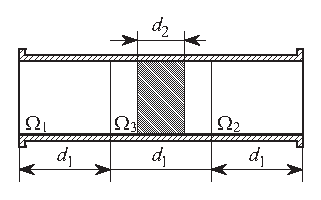
\includegraphics[scale = 0.925]{figs/slabgeo.eps}
  \caption{Test case of a dielectric slab of thickness $d_2$ in a rectangular
  waveguide.}
  \label{f:slabgeo}
\end{figure}
The diameter of the slab is $d_2 = 7~\operatorname{mm}$.
The field domain is longitudinally subdivided into 3 subdomains,
each of length $d_1 = 9~\operatorname{mm}$.
A FE discretization results in a full model of dimension 28825.
Applying the DD approach gives for the dimension of \eqref{eq:lastDomParam} a reduced size of 10348.
We consider as system response the reflection coefficient $S_{11}$ as a function
of frequency and the electric permittivity and magnetic permeability of the slab.
The parameters vary in the ranges $f = 7 \dots 13~\operatorname{GHz}$,
$\varepsilon_r = (1 \dots 7) - 0.01j$ and $\mu_r = 1 \dots 7$.
A ROM is constructed from the solutions at the parameter points given by the tensor product of
$f = \{7,10,13\}~\operatorname{GHz}$, $\varepsilon_r = \{1,3,5,7\}$ and $\mu_r = \{ 1,3,5,7 \}$.
This choice results in a ROM dimension of $p = 2 \times (3 \times 4 \times 4) = 96$,
where the factor two arises from the existence of two ports.
Even though the resulting ROM is constructed from pure lossless solutions,
small dielectric losses can be taken into account very accurately.
Using the lossless solution vectors as projection vectors,
renders the ROM real,
and therefore allows a faster model evaluation.
Figs. \ref{f:slab_mu2} and \ref{f:slab_mu6} show the results for two dimensional cuts
through the three dimensional response hypersurface at $\mu_r = 2$ and $\mu_r = 6$.
%
\begin{figure}[!t]
  \centering
  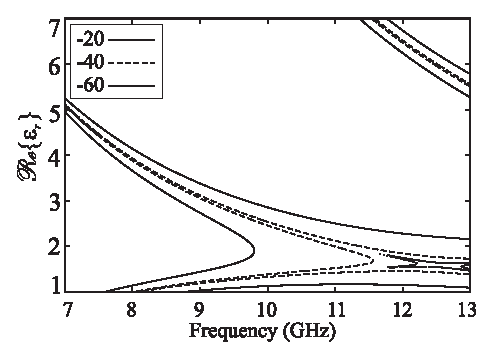
\includegraphics[scale = 0.925]{figs/slab_mu2.eps}
  \caption{Reflection coefficient magnitude $|S_{11}|$ in dB at $\mu_r = 2$ as a function of $f$ and $\varepsilon_r$.}
  \label{f:slab_mu2}
\end{figure}
\begin{figure}[!t]
  \centering
  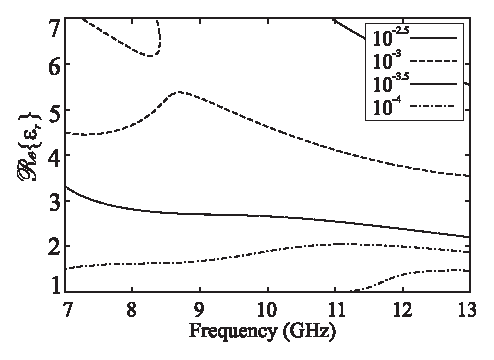
\includegraphics[scale = 0.925]{figs/slab_mu2_error.eps}
  \caption{Magnitude of error in reflection coefficient \eqref{eq:ErrorDef}
    at $\mu_r = 2$ as a function of $f$ and $\varepsilon_r$.}
  \label{f:slab_mu2_error}
\end{figure}
%
Each figure consists of $301 \times 301$ points,
which corresponds to 90601 model evaluations.
To assess the accuracy of the ROM,
we consider the magnitude of the error in reflection coefficient $|\text{Error }S_{11}|$,
%
\begin{equation} \label{eq:ErrorDef}
  |\text{Error }S_{11}| = |S_{11}^{ROM} - S_{11}^{ref}|
\end{equation}
%
where the analytical solution is taken as reference $S_{11}^{ref}$.
Figs. \ref{f:slab_mu2_error} and \ref{f:slab_mu6_error} depict $|\text{Error }S_{11}|$ at $\mu_r = 2$ and $\mu_r = 6$.
%
\begin{figure}[!t]
  \centering
  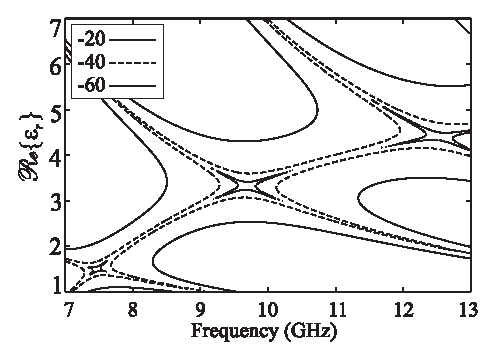
\includegraphics[scale = 0.925]{figs/slab_mu6.eps}
  \caption{Reflection coefficient magnitude $|S_{11}|$ in dB at $\mu_r = 6$ as a function of $f$ and $\varepsilon_r$.}
  \label{f:slab_mu6}
\end{figure}
%
\begin{figure}[!t]
  \centering
  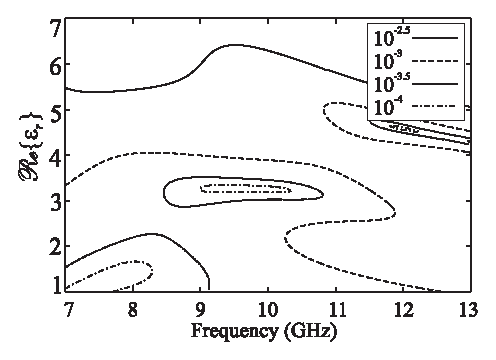
\includegraphics[scale = 0.925]{figs/slab_mu6_error.eps}
  \caption{Magnitude of error in reflection coefficient \eqref{eq:ErrorDef}
    at $\mu_r = 6$ as a function of $f$ and $\varepsilon_r$.}
  \label{f:slab_mu6_error}
\end{figure}
%
It is important to notice,
that the error is taken compared to the analytical solution.
Numerical experiments show,
that a further increase in the dimension of the ROM doesn't lead to a reduction of the error.
Therefore we can conclude that the main contribution of the error is from the FE approximation of the original model,
not from the order reduction step.
Table \ref{tab:runtimes} reports the computation times for the proposed ROM approach,
a straight forward FE implementation and the DD method alone (FEM+DD).
The evaluation of the ROM is two to three orders of magnitude faster than that of the two other models.
For the two dimensional cuts of Figs. \ref{f:slab_mu6} and \ref{f:slab_mu2}
this results in a reduction of running time from 25 hours (FEM) and 13 hours (FEM+DD) to less than three minutes.
Comparing the time for generating the ROM,
an acceleration of roughly forty percent by incorporating the DD approach is observed.

%\begin{figure}[!t]
%  \centering
%  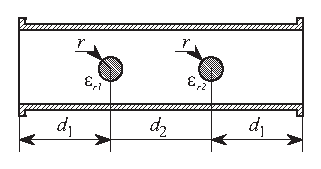
\includegraphics{figs/twopostsgeo.eps}
%  \caption{Waveguide section comprising two posts of radius $r$
%  placed in the middle of the waveguide at a mutual
%  distance $d_2$.}
%  \label{f:twopostsgeo}
%\end{figure}


\subsection{Four posts}

As a second example we consider the WR90 waveguide comprising four dielectric posts
with radius $r = 4~\operatorname{mm}$ and
distances $d_1 = d_2 = d_3 = 20~\operatorname{mm}$
shown in Fig. \ref{f:fourpostsgeo}.
\begin{figure}[!t]
  \centering
  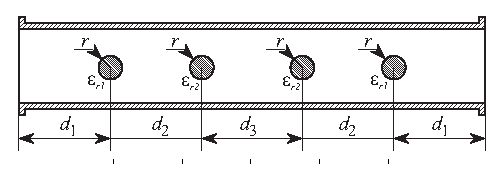
\includegraphics[scale = 0.925]{figs/fourpostsgeo.eps}
  \caption{Waveguide section comprising four posts of radius $r$
  placed in the middle of the waveguide at mutual distances $d_2$ and $d_3$.}
  \label{f:fourpostsgeo}
\end{figure}
A FE discretization results in a full model with 39813 degrees of freedom.
For a given frequency,
the DD approach gives for \eqref{eq:lastDomParam} a dimension of 9204.
We again consider as system response the reflection coefficient $S_{11}$,
now as a function of the frequency and
the relative dielectric permittivities $\varepsilon_{r1}$ and $\varepsilon_{r2}$ shown in Fig. \ref{f:fourpostsgeo}.
The parameter ranges are $f = 7 \dots 13~\operatorname{GHz}$,
$\varepsilon_{r1} = (1 \dots 26) - 0.01j$ and $\varepsilon_{r2} = (1 \dots 26) - 0.01j$.
%According to \eqref{eq:ProjVecEqSolVec},
The projection matrix spans the solution space at the parameter points given by the the tensor product of
$f = \{7,9,11,13\}~\operatorname{GHz}$ and $\varepsilon_{r1} = \varepsilon_{r2} =\{1, 7.25, 13.5, 19.75, 26\}$.
Since again we consider two ports,
with one mode at each,
this results in a ROM dimension of $p = 2 \times (4 \times 5 \times 5) = 200$.
Fig. \ref{f:sixslices} shows various slices through the response hypersurface at
$\varepsilon_{r2} = \{1,6,11,16,21,26\} - 0.01j$.
\begin{figure*}[!t]
  \centering
  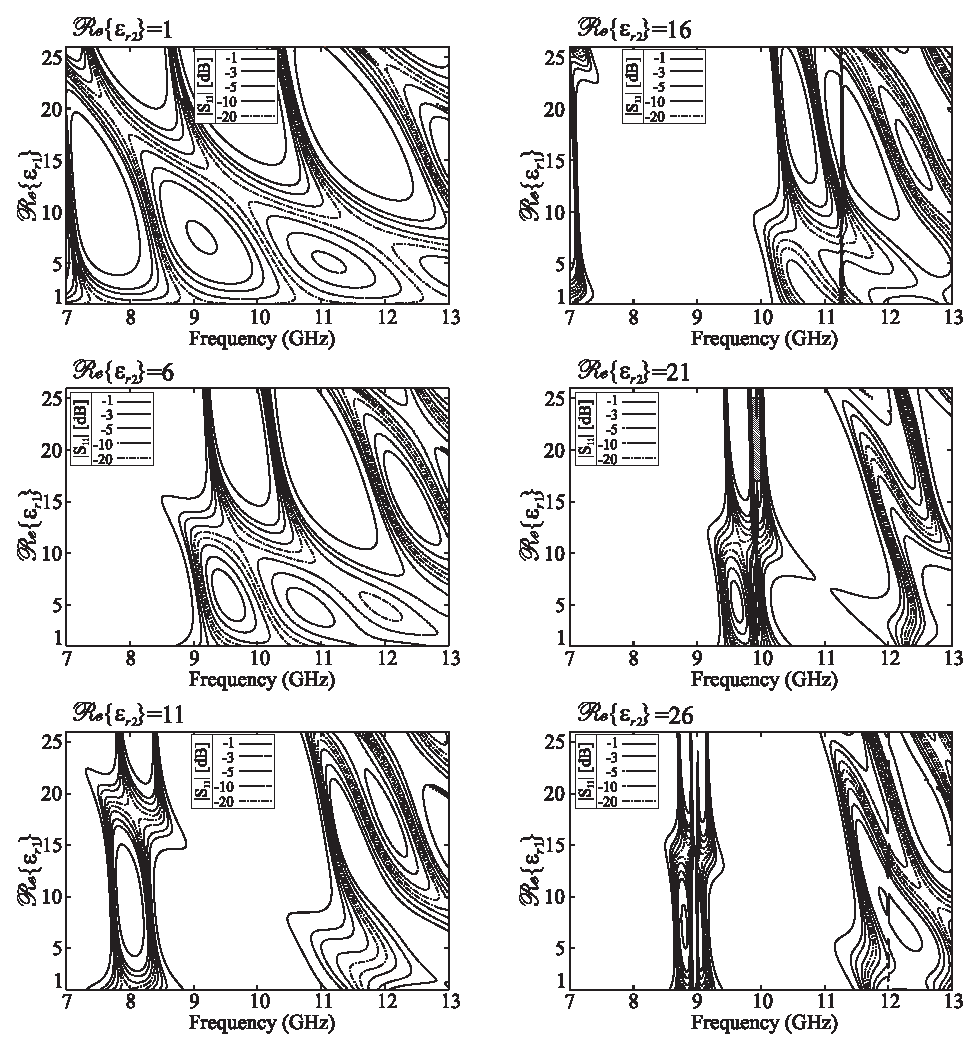
\includegraphics[scale = 0.925]{figs/sixslices.eps}
  \caption{Lines at equal values of the reflection coefficient (dB) for
  the four posts filter. $\varepsilon_{r2}$ assumes the discrete values
  $1,6,11,16,21,26$ while $\varepsilon_{r1}$ is sampled over 251 points in the
  $[1,26]$ range and 601 frequency points are taken in the
 $[7,13]~\operatorname{GHz}$ range. }
  \label{f:sixslices}
\end{figure*}
Each subplot consists of $601 \times 251 = 150851$ model evaluations.
For the present structure,
no analytical solution is available.
To investigate the accuracy of the ROM,
we therefore have to compute the reference values $S_{11}^{ref}$ in \eqref{eq:ErrorDef} with full FE simulations.
Since such calculations are very time consuming,
we are unable to show comparisons for the two dimensional cuts of Fig. \ref{f:sixslices}.
Instead,
we are considering lines along the frequency axis for constant values of $\varepsilon_{r1}$ and $\varepsilon_{r2}$.
Fig. \ref{f:fourPostsError} depicts the error for four points in the $(\varepsilon_{r1},\varepsilon_{r2})$-space.
\begin{figure}[!t]
  \centering
  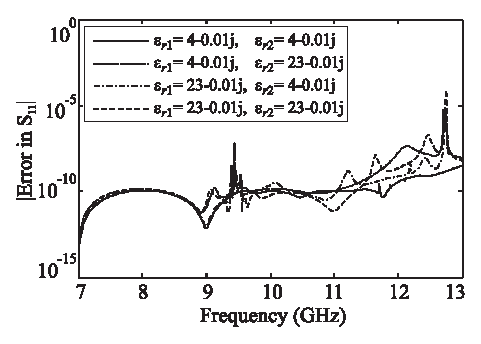
\includegraphics[scale = 0.925]{figs/fourPostsError.eps}
  \caption{Magnitude of error in reflection coefficient as a function of frequency.}
  \label{f:fourPostsError}
\end{figure}
Note, $\varepsilon_{r1}$ and $\varepsilon_{r2}$ are chosen such that
they lie in the outer region of the parameter space and in the middle of two expansion points.
This is where the greatest ROM errors occur.
In most parts of the parameter domain,
the error is in the range of $10^{-12}$ to $10^{-8}$,
the maximum error is in the order of $10^{-4}$,
which usually is lower than the FE approximation error.

Fig. \ref{f:slicezoom} shows a zoom into the hatched region of the two dimensional cut at $\operatorname{Re} \{ \varepsilon_{r2} \} = 21$
in Fig. \ref{f:sixslices}.
\begin{figure}[!t]
  \centering
  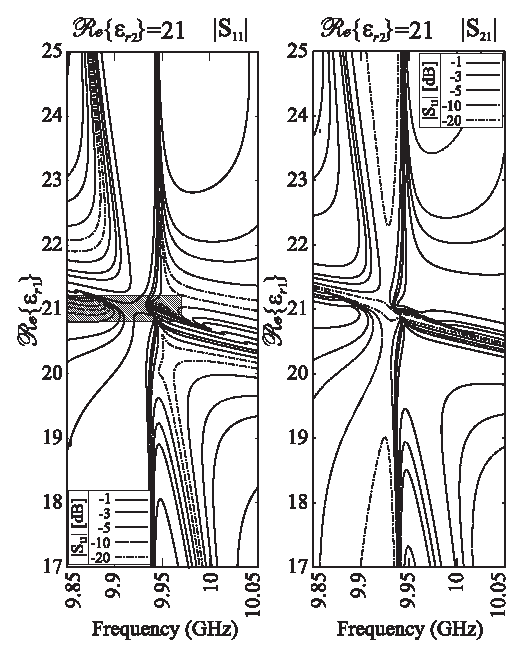
\includegraphics[scale = 0.925]{figs/slicezoom.eps}
  \caption{Lines at equal values of the reflection coefficient (dB) for
  the four posts filter. The area corresponds to the hatched area in
  Fig. \ref{f:sixslices}, second row right.}
  \label{f:slicezoom}
\end{figure}
Even with such a rather simple structure,
one can observe very narrowband resonance phenomena.
This underlines the importance of the very fine resolution in the parametric sweeps,
which is affordable by using MOR.
A further zoom into the hatched region of Fig. \ref{f:slicezoom} shown in Figs. \ref{f:filterstop} and \ref{f:filterpass} demonstrate,
that within a difference of $\Delta \varepsilon_{r1} = 0.19$
the considered structure behaves like a passband or a stopband filter.
\begin{figure}[!t]
  \centering
  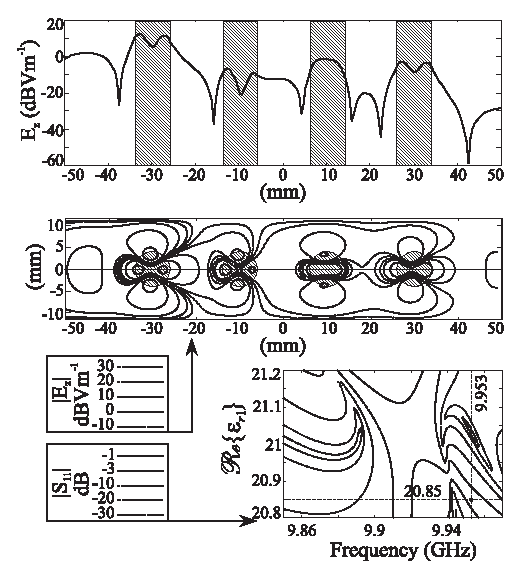
\includegraphics[scale = 0.925]{figs/filterstop.eps}
  \caption{Lines at equal values of the field amplitude on an $y=constant$
  cut (middle). On top of the figure the field amplitude is reported
  as a conventional 2D plot along the longitudinal axis of the device. Posts are
  shown as hatched areas. On the bottom the working point of the device is highlighted,
  in a zoom of Fig.~\ref{f:slicezoom}, and legends are reported.}
  \label{f:filterstop}
\end{figure}
\begin{figure}[!t]
  \centering
  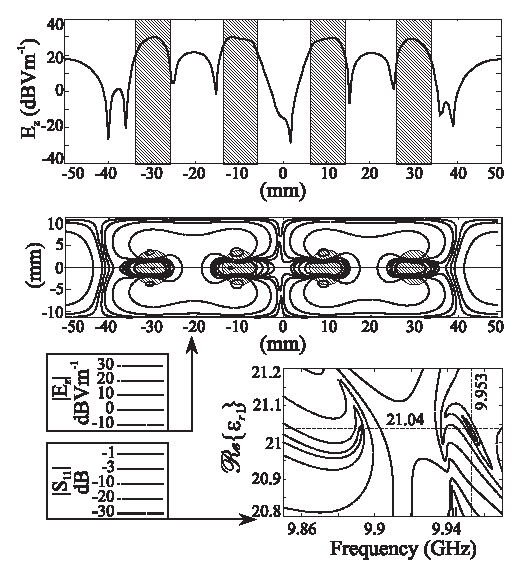
\includegraphics[scale = 0.925]{figs/filterpass.eps}
  \caption{Lines at equal values of the field amplitude on an $y=constant$
  cut (middle). On top of the figure the field amplitude is reported as a
  conventional 2D plot along the longitudinal axis of the device. Posts are
  shown as hatched areas. On the bottom the working point of the device is highlighted,
  in a zoom of Fig.~\ref{f:slicezoom}, and legends are reported.}
  \label{f:filterpass}
\end{figure}
\begin{footnotesize}
\begin{table}
    \centering
    \caption{Computational times, in seconds.} \label{tab:runtimes} %\vspace{-3mm}
    \begin{tabular}{r|cc|cc}
    \multicolumn{ 5}{c}{\bf Evaluation} \\
     \hline  \hline
    \multicolumn{ 1}{c}{} & \multicolumn{2}{|c|}{Dielectric slab} & \multicolumn{2}{c}{Dielectric posts} \\
    &	per sample & total & per sample & total \\
    \hline
    FEM & $0.975$ & $8.83\times10^{4}$ & $1.419$ & $2.14\times10^{5}$  \\
    FEM+DD & $0.512$ & $4.64\times10^{4}$ &  $0.854$ & $1.29\times10^{5}$  \\
    MOR & $1.89\times10^{-3}$ & $171.7$ & $9.95\times10^{-3}$  & $1.50\times10^{3}$  \\
    \hline \hline
    \multicolumn{5}{c}{\;} \\
    \multicolumn{ 5}{c}{\bf ROM Generation} \\
    \hline \hline
    & \multicolumn{2}{|c|}{total} & \multicolumn{2}{c}{total} \\
    \hline
    FEM & \multicolumn{2}{|c|}{55.2} & \multicolumn{2}{c}{168} \\
    FEM+DD & \multicolumn{2}{|c|}{33.0} & \multicolumn{2}{c}{111} \\
    \hline \hline
    \end{tabular}
%\vspace{-3mm}
\end{table}
\end{footnotesize}

%\begin{table}
%    \centering
%    \caption{Computational results.} \label{tab:runtimes} %\vspace{-3mm}
%    \begin{tabular}{|c|c|r|c|r|}
%    \hline
%    \multicolumn{ 5}{|c|}{Evaluation} \\
%    \hline
%    \hline
%    \multicolumn{ 1}{|c|}{} & \multicolumn{2}{|c|}{Dielectric slab} & \multicolumn{2}{|c|}{Dielectric posts} \\
%    \hline
%    &	per sample (s) & total (s) & per sample (s) & total (s) \\
%    \hline
%    \multicolumn{ 1}{|c|}{FEM} & 0.974991 & 88335.2 & 1.41885 & 214035 \\
%    \hline
%    \multicolumn{ 1}{|c|}{FEM+DD} & 0.512207 & 46406.5 &  0.853774 & 128793 \\
%    \hline
%    \multicolumn{ 1}{|c|}{MOR} & 1.89497e-3 & 171.6866 & 9.94745e-3 & 1500.58 \\
%    \hline
%    \hline
%    \multicolumn{ 5}{|c|}{ROM Generation} \\
%    \hline
%    \hline
%    & \multicolumn{2}{|c|}{total} & \multicolumn{2}{|c|}{total} \\
%    \hline
%    FEM & \multicolumn{2}{|c|}{55.206} & \multicolumn{2}{|c|}{167.93} \\
%    \hline
%    FEM+DD & \multicolumn{2}{|c|}{32.992} & \multicolumn{2}{|c|}{111.42} \\
%    \hline
%    \end{tabular}
%%\vspace{-3mm}
%\end{table}

Table \ref{tab:runtimes} reports that the speed up in model evaluation
using our order reduction approach is two orders of magnitude.
%Thus reducing the time for computing one two dimensional slice if Fig. \ref{f:sixslices}
%from 60 hours (FEM) and 36 hours (FEM+DD) to approximately 25 minutes.
The incorporation of the DD method again reduces ROM generation time by roughly 34 percent.


\section{Conclusions}

In this paper we have presented a combined DD-MOR approach for parametric FE analysis of passive microwave structures.
The incorporation of the DD into the ROM generation process allows the efficient use of multipoint MOR methods,
since a new projection vector can be computed at the cost of solving one single subdomain.
The numerical examples demonstrate the usefulness of this technique.

Future work will focus on applying this approach onto geometry parameters,
%which do not enter the FE system in explicit form,
and the use of such parametric ROMs in optimization scenarios.


\bibliographystyle{IEEEtran}
\bibliography{IEEEabrv,IEEE_Saar_v0.5}

% biography section
%
% If you have an EPS/PDF photo (graphicx package needed) extra braces are
% needed around the contents of the optional argument to biography to prevent
% the LaTeX parser from getting confused when it sees the complicated
% \includegraphics command within an optional argument. (You could create
% your own custom macro containing the \includegraphics command to make things
% simpler here.)
%\begin{biography}[{\includegraphics[width=1in,height=1.25in,clip,keepaspectratio]{mshell}}]{Michael Shell}
% or if you just want to reserve a space for a photo:

%\begin{IEEEbiography}{Michael Shell}
%Biography text here.
%\end{IEEEbiography}



% that's all folks
\end{document}
